\documentclass{book}
%\documentclass{article}                            %for shorter notes
\usepackage{graphicx}                              %for PNG images (pdflatex)
%\usepackage{graphics}                              %for EPS images (latex)
\usepackage[linkbordercolor={1.0 1.0 0.0}]{hyperref} %for \url tag
\usepackage{color}                                 %for defining custom colors
\usepackage{framed}                                %for shaded and framed paragraphs
\usepackage{textcomp}                              %for various symbols, e.g. Registered Mark
\usepackage{geometry}                              %for defining page size
\usepackage{longtable}                             %for breaking tables
%
\geometry{verbose,a4paper,tmargin=2.5cm,bmargin=2.5cm,lmargin=2.5cm,rmargin=2cm}
\hypersetup{
  pdfauthor = {Author Name},
  pdftitle = {Paper title},
  pdfsubject = {Paper subject},
  pdfkeywords = {Paper,keyword,comma-separated},
  pdfcreator = {PDFLaTeX with hyperref package},
  pdfproducer = {PDFLaTeX}
}
%
\bibliographystyle{IEEEtran}                       %a nice bibliography style
%
\def\efill{\hfill\nopagebreak}%
\hyphenation{Nordu-Grid}
\setlength{\parindent}{0cm}
\setlength{\FrameRule}{1pt}
\setlength{\FrameSep}{8pt}
\addtolength{\parskip}{5pt}
\renewcommand{\thefootnote}{\fnsymbol{footnote}}
\renewcommand{\arraystretch}{1.3}
\newcommand{\dothis}{\colorbox{shadecolor}}
\newcommand{\globus}{Globus Toolkit\textsuperscript{\textregistered}~2~}
\newcommand{\GT}{Globus Toolkit\textsuperscript{\textregistered}}
\newcommand{\ngdl}{\url{http://ftp.nordugrid.org/download}~}
\newcommand{\ACC}{\texttt{ACC}}
\newcommand{\TargetGenerator}{\texttt{TargetGenerator}}
\newcommand{\TargetRetriever}{\texttt{TargetRetriever}}
\newcommand{\ExecutionTarget}{\texttt{ExecutionTarget}}
\newcommand{\Broker}{\texttt{Broker}}
\newcommand{\Submitter}{\texttt{Submitter}}
\newcommand{\JobDescription}{\texttt{JobDescription}}
\newcommand{\JobSupervisor}{\texttt{JobSupervisor}}
\newcommand{\JobController}{\texttt{JobController}}
\newcommand{\Job}{\texttt{Job}}
\newcommand{\UserConfig}{\texttt{UserConfig}}
\newcommand{\ClientInterface}{\texttt{ClientInterface}}
\definecolor{shadecolor}{rgb}{1,1,0.6}
\definecolor{salmon}{rgb}{1,0.9,1}
\definecolor{bordeaux}{rgb}{0.75,0.,0.}
\definecolor{cyan}{rgb}{0,1,1}
%
%----- DON'T CHANGE HEADER MATTER
\begin{document}
\def\today{\number\day/\number\month/\number\year}

\begin{titlepage}

\begin{tabular}{rl}
\resizebox*{3cm}{!}{
\includegraphics{ng-logo.png}}
&\parbox[b]{2cm}{\textbf \it {\hspace*{-1.5cm}NORDUGRID\vspace*{0.5cm}}}
\end{tabular}

\hrulefill

%-------- Change this to NORDUGRID-XXXXXXX-NN

{\raggedleft NORDUGRID-XXXXXXX-NN\par}

{\raggedleft \today\par}

\vspace*{2cm}

%%%%---- The title ----
{\centering \textsc{\Large Paper title}\Large \par}
\vspace*{0.5cm}
    
%%%%---- A subtitle, if necessary ----
{\centering \textit{\large Paper subtitle}\large \par}
    
\vspace*{1.5cm}
%%%%---- A list of authors ----
    {\centering \large Paper author\footnote{authors@address} \large \par}
    
%%%%---- An abstract - if style is article ----
%\begin{abstract}
%The abstract
%\end{abstract}
\end{titlepage}

\tableofcontents                          %Comment if use article style
\newpage
\chapter{Preface}
\label{sec:intro}

This document describes from a technical viewpoint a plugin based client library for the new 
Web Service (WS) based Advanced Resource Connector (ARC) middleware. The library consists of 
a set of C++ classes for 

\begin{itemize}
\item{handling proxy, user and host certificates,}
\item{performing resource discovery and information retrieval,}
\item{job submission and management and}
\item{data handling.}
\end{itemize}

All capabilities are enabled for three different grid flavours (Production ARC, ARC1 and gLite) 
through the modular design using plugins specialized for each supported middleware. Future 
extensions to support additional middlewares involve plugin compilation only i.e. no recompilation 
of main libraries or client.

Using the library a set of command line tools have been built which puts the library's functionality 
at the fingertips of users. While this documentation will illustrate how such command line tool can be 
built, the main documention of the command line tools is given in the client user manual [ref].

In the following we will give a functionality overview in Section~\ref{sec:FuncOver} while all technical 
details will be given in Section~\ref{sec:Implementation}. Section~\ref{sec:cli} will through examples 
show how command line interfaces can be built upon the library.

\chapter{Functionality Overview}
\label{sec:FuncOver}
The new ARClib makes extensive use of plugins for command handling. These plugins are handled by a set 
of higher level classes which thus are the ones to offer the plugin functionality to external calls. In 
this section an overview of the library's main functionality is given which also introduces the most 
important higher level classes.
\section{Resource Discovery and Information Retrieval}
\label{sec:TargetDiscovery}
With the increasing number of grid clusters around the world, a reliable and fast resource discovery and 
information retrieval capability is of crucial importance for a user interface. The new ARClib resource 
discovery and information retrieval component consists of three classes; The {\TargetGenerator}, the 
{\TargetRetriever} and the {\ExecutionTarget}. Of these the {\TargetRetriever} is a base class for further grid 
middleware specific specialization (plugin).

Figure \ref{fig:ResDisc} depicts how the classes work together in a command chain to discover all resources 
registered with a certain information server. Below a description of each step is given:

\begin{figure}[ht]
\centering{{\scalebox{0.75}{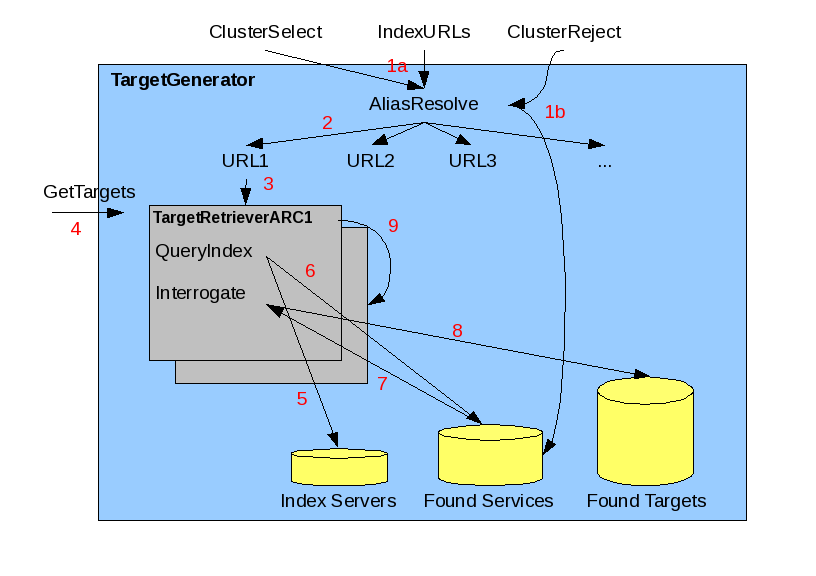
\includegraphics{TargetDiscovery.png}}}
\caption{\label{fig:ResDisc}Diagram depicting the process of resource discovery and information retrieval.} }
\end{figure}

\begin{enumerate}
\item{The {\TargetGenerator} takes three URL arrays as input. First array contains individually selected computing services, while the 
second array contains individually selected index servers (1a). The last array contains a list of rejected services. This 
list is parsed through alias resolve before being inserted as filter to the storage of found services (1b).}
\item{The complete list of URLs pointing to computing services and index servers.}
\item{For each URL a {\TargetRetriever} plugin is loaded using the ARC loader. The {\TargetRetriever} is initialized 
with the URL and the information about this URL pointing to a computing service or an index server.}
\item{An external call is received calling for targets to be prepared. Call is propagated to all loaded {\TargetRetriever}s.}
\item{The call for targets is processed by each {\TargetRetriever} in parallel. If the {\TargetRetriever} is initialized with an 
index server URL it first registers at the Index Servers store kept by the {\TargetGenerator}. If allowed to register, the index 
server is queried and the query result processed.}
\item{The TargetRetriver finds a registered service and contacts the Found Services store kept by the {\TargetGenerator} to check 
if the service in question has been found be another {\TargetRetriever}. (Services often registers at more than one index server, 
thus different {\TargetRetriever}s may discover the same service.)}
\item{If the {\TargetGenerator} allows registration in the Found Services store, the {\TargetRetriever} progresses to interrogate the service.}
\item{Found and processed {\ExecutionTarget}s are stored in the Found Targets store kept by the {\TargetGenerator} for later usage 
(e.g. status printing or job submission).}
\item{Index servers often registers with other index servers creating a nested hierarchical information structure. For this 
reason a {\TargetRetriever} processing the query result from an index server may encounter other index servers. In such
events the {\TargetRetriever} will call itself recursively creating a new thread for the new URL. This ensures optimum speed and 
performance for resource discovery.}
\end{enumerate}

The example above outlines how the {\TargetRetriever} works when initialized with an URL pointing to and index server. However, 
as indicated it also accepts initialization with a service URLs, in which case the {\TargetRetriever} will try to register the 
service in the {\TargetGenerator} Found Services store. If allowed the {\TargetRetriever} will progress with the target interrogation 
method.

\section{Job Submission}
\label{sec:JobSubmission}
Job submission starts with the resource discovery and target preparation as outlined in the Section~\ref{sec:TargetDiscovery}. 
Not until a list of possible targets (which allows the user) is available is the job description read in order to enable bulk 
job submission of widely different jobs without having to reperform the resource discovery. In addition to the classes mentioned 
above the job submission makes use of the {\Broker}, {\JobDescription} and {\Submitter} classes. At the time of writing the {\Broker} is 
not implemented, but it's functionality and interface is well known, and thus we will include it in the overview given here.
The {\Submitter} is base class for further grid middleware specific specialization (plugin) similarly to the {\TargetRetriever}.

\begin{figure}[ht]
\centering{{\scalebox{0.75}{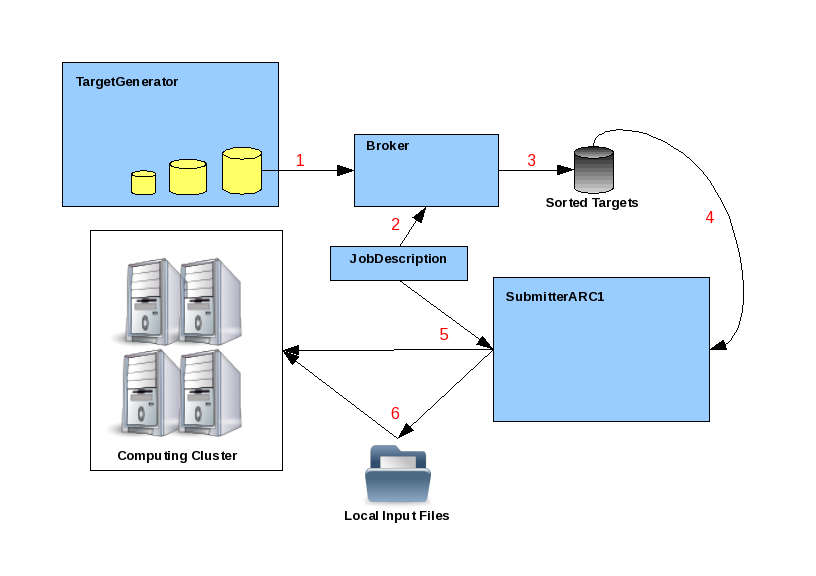
\includegraphics{JobSubmission.png}}}
\caption{\label{fig:JobSub}Diagram depicting the process of submitting a job to a computing service.}}
\end{figure}

Figure \ref{fig:JobSub} shows a job submission sequence and below a description of each step is given:

\begin{enumerate}
\item{The {\TargetGenerator} has prepared a list of {\ExecutionTarget}s. Depending on the URLs provided to the {\TargetGenerator} the list of 
found {\ExecutionTarget}s may be empty or contain several targets. Targets may even represent more than one grid flavour. The list of 
found targets are given as input to the {\Broker}.}
\item{In order to rank the found services ({\ExecutionTarget}s) the {\Broker} needs detailed knowledge about the job requirements, thus the 
{\JobDescription} is passed as input to the brokering process.}
\item{The {\Broker} outputs a ordered list of {\ExecutionTarget}s according to the provided {\JobDescription}.}
\item{Each ExectionTarget has a method to return a specialized {\Submitter} which is capable of submitting jobs to the service it 
represents. The best suitable {\ExecutionTarget} for the job is asked to return a {\Submitter} for job submission.}
\item{The {\Submitter} takes the {\JobDescription} as input and uploads it to the computing service.}
\item{The {\Submitter} identifies local input files from the {\JobDescription} and uploads them to the computing service.}
\end{enumerate}

\section{Job Management}
Information about active jobs is stored in a local xml file which is used for later job management. As this file may contain 
information about jobs running on completely different grid flavours, job management should be handled using plugins similar to 
resource discovery and job submission. The following classes are used:

\section{Data Handling}
\label{sec:DataHandling}

\chapter{Implementation}
\label{sec:Implementation}
Clever text here.
\section{Generic Classes}
\subsection{{\ACC}}

\subsection{{\TargetGenerator}} The {\TargetGenerator} class is the main class for resource discovery and information retrieval. It loads 
{\TargetRetriever} plugins in accordance with the input URLs using the ARC Loader (e.g. if an URL pointing to an ARC1 resource is given 
the TargetRetrieverARC1 is loaded).

To perform a resource discovery, first construct a {\TargetGenerator} object using the {\TargetGenerator} constructor,

\begin{shaded}
\begin{verbatim}
TargetGenerator(const std::list<std::string>& clusterselect,
                const std::list<std::string>& clusterreject,
                const std::list<std::string>& indexurls);
\end{verbatim}
\end{shaded}

where \texttt{clusterselect}, \texttt{clusterreject} and \texttt{indexurls} are lists of strings where each string is either 
an URL or a regular string defined as an alias in the user (or system) configuration. Without any further explanation it is 
hard to decode from an URL if it points to a index server or computing service of a certain grid flavour. Thus in order for 
the {\TargetGenerator} to know which {\TargetRetriever} should be loaded URLs have to be given in a format where the grid 
flavour preceeds the actual URL, e.g:

\begin{shaded}
\begin{small}
\begin{verbatim}
ARC0:ldap://grid.tsl.uu.se:2135/mds-vo-name=sweden,O=grid
ARC0:ldap://grid.tsl.uu.se:2135/nordugrid-cluster-name=grid.tsl.uu.se,Mds-Vo-name=local,o=grid
\end{verbatim}
\end{small}
\end{shaded}

where the former is the URL to an index server while the latter is an URL to a computing service.

To prepare a list of {\ExecutionTarget}s use the {\TargetGenerator} object and invoke its method

\begin{shaded}
\begin{verbatim}
GetTargets(int targetType, int detailLevel);
\end{verbatim}
\end{shaded}

The {\TargetGenerator} will pass this request to the loaded {\TargetRetriever}s running them as individual threads 
for improved performance. The {\TargetGenerator} keeps records of by {\TargetRetriever} found index servers and computing 
services in order to avoid multiple identical queries. Accepted {\ExecutionTarget}s are stored in the FoundTargets 
array kept by the {\TargetGenerator}. See also Section~\ref{sec:TargetDiscovery} for a schematic drawing of the 
resource discovery process.

Information about the found {\ExecutionTarget}s can be printed by 

\begin{shaded}
\begin{verbatim}
PrintTargetInfo(bool longlist) const;
\end{verbatim}
\end{shaded}

\subsection{{\TargetRetriever}} The {\TargetRetriever} is base class for {\TargetRetriever} grid middleware specializations and 
inherits from the \texttt{ACC} base class in order to be loadable by the ARC \texttt{Loader}. It is designed to work on conjunction 
with the {\TargetGenerator} contains and contains the pure virtual method

\begin{shaded}
\begin{verbatim}
virtual void GetTargets(TargetGenerator& mom, int targetType,
                        int detailLevel) = 0;
\end{verbatim}
\end{shaded}

which is to be implemented by the specialized class. While it is not mandatory it is recommended that the specialized class 
divides this method into two components: QueryIndex and InterrogateTarget. The former is handles index server queries, and the 
latter the computing service queries and {\ExecutionTarget} preparation. 

If an index server query yields an url to a different index server then the one queried, then the {\TargetRetriever} should 
call itself recursively creating a new {\TargetRetriever} for the discovered index server. 

\subsection{{\ExecutionTarget}} The {\ExecutionTarget} is the class representation of a computing resource (queue) capable of 
executing a grid job. It serves as input to the {\Broker} which is foreseen to be able to select between different 
{\ExecutionTarget}s from different grid flavours without apriori knowing their difference. The {\ExecutionTarget} class 
mimics the glue2 information model (with a flattened structure), and thus a mapping between attributes from other information 
systems into the glue2 format is needed.  Appendix XX shows the current mapping for the production ARC, ARC1 and gLite middlewares. 

All attributes of the {\ExecutionTarget} can be printed by the method

\begin{shaded}
\begin{verbatim}                                                                                                                            
void Print(bool longlist) const;
\end{verbatim}
\end{shaded}

Following a broker decision jobs are to be submitted. Since all information about the selected computing service resides within the 
selected {\ExecutionTarget}, the {\ExecutionTarget} is capable of returning a {\Submitter} capable of submitting a 
job to the service which is represents.

\begin{shaded}
\begin{verbatim}
Submitter *GetSubmitter() const;
\end{verbatim}
\end{shaded}

\subsection{{\Broker}} The {\Broker} is not yet implemented and thus not described here.

\subsection{{\JobDescription}} When addressing interoperability it is of paramount importance to transparently address grid job 
descriptions written in different job description languages by translating them automatically. In the ARClib library this functionality 
is implemented in the {\JobDescription} class. This is a generic class that takes a job description (string )as input 

\begin{shaded}
\begin{verbatim}
setSource( const std::string source ) throw(JobDescriptionError);
\end{verbatim}
\end{shaded}

in any supported formats (currently xRSL, JDL, JSDL), converts and stores it in a JSDL-like internal job description format. The identification 
of the source's description format is internally handled by a \texttt{JobDescriptionOrderer} class which identifies the format by pattern
matching.

Different operations, like getting the job description in other formats or getting job-related information, can be performed using the 
description-independent functions of this class, e.g.:

\begin{shaded}
\begin{verbatim}
getProduct(std::string& product, std::string format="JSDL") throw(JobDescriptionError);
\end{verbatim}
\end{shaded}

The {\JobDescription} class has tree back-end classes, sometimes referred to as back-end or translator modules, corresponding to the three 
supported job description languages. The {\JobDescription} class chooses the appropriate back-end module according to the pattern match 
performed by the \texttt{JobDescriptionOrderer}, and uses the back-end module for parsing and generating the job descriptions.

\subsection{{\Submitter}} {\Submitter} is base class for grid specific specializations (plugin). It submits job(s) to the service 
it represents and uploads (by the job needed) local input files. 

\begin{shaded}
\begin{verbatim}
virtual bool Submit(JobDescription& jobdesc, XMLNode& info) = 0;
\end{verbatim}
\end{shaded}

The \texttt{Submit} method fills the XML node \texttt{info} with all needed information about the job for later job management. 
The {\Submitter} is returned by the {\ExecutionTarget} selected for job execution and thus the {\ExecutionTarget} populates 
(through XML config element) the {\Submitter} with information about submission endpoint (URL) and job description languages 
``spoken'' by the target.

\subsection{{\JobSupervisor}} The {\JobSupervisor} is responsible for loading the appropriate {\JobController}s for managing 
jobs running on a certain grid flavour. Job manipulation can be performed either on individual jobs or on groups of jobs (e.g. 
all jobs running on certain cluster or all jobs with job state ``FINISHED''), and in order to translate the by user given 
information into a set of loadable {\JobController}s the {\JobSupervisor} makes extensive use of the local XML file housing 
information about all active jobs. Thus the {\JobSupervisor} constructor becomes

\begin{shaded}
\begin{verbatim}
JobSupervisor(const std::list<std::string>& jobs,
              const std::list<std::string>& clusterselect,
              const std::list<std::string>& clusterreject,
              const std::string joblist);
\end{verbatim}
\end{shaded}

where \texttt{jobs} is a list of job identification strings (jobids), \texttt{clusterselect} is a list of selected computing services, 
\texttt{clusterreject} is a list of rejected computing services and \texttt{joblist} is a string pointing to the local XML file 
with job information. Syntax for \texttt{clusterselect} and \texttt{clusterreject} is identical to the one used by the {\TargetGenerator}
for for internal consistency.

Although being loaded by the {\JobSupervisor} the {\JobController} objects truly resides within the ARC Loader which is a member 
of the {\JobSupervisor} class. In order to get handles on the {\JobController}s the inline method

\begin{shaded}
\begin{verbatim}
std::list<Arc::JobController*> GetJobControllers(){return JobControllers;}
\end{verbatim}
\end{shaded}

returns a list of pointers to the loaded {\JobController}s.

\subsection{{\JobController}} The {\JobController} is both base class for grid specific specializations, but also the implementor of all 
public functionality offered by the {\JobController}s. In other words all virtual functions of the {\JobController} are private. The 
initialization of a (specialized) {\JobController} object takes two steps. First the constructor has to invoked

\begin{shaded}
\begin{verbatim}
JobController(Arc::Config *cfg, std::string flavour);
\end{verbatim}
\end{shaded}

This is usually done by the ARC Loader which sees to that the {\JobController} receives information about its flavour (grid) and 
the local XML file containing information about all active jobs (flavour independent). Next step is the filling of the {\JobController}'s
job pool \texttt{JobStore} which is the pool of jobs that the {\JobController} can manage.

\begin{shaded}
\begin{verbatim}
void FillJobStore(std::list<std::string> jobs,
                  std::list<std::string> clusterselect,
                  std::list<std::string> cluterreject);
\end{verbatim}
\end{shaded}

Here \texttt{jobs}, \texttt{clusterselect} and \texttt{clusterreject} have the same interpretation as in the {\JobSupervisor} constructor. 
However, while the latter only had to identify which {\JobController}s should be loaded, the {\JobController} itself has to decode the 
supplied lists into a list of jobs with non-overlapping entries which will be filled into the JobStore. Due to possible conflicts 
within the supplied lists, rules have to be set up for dealing with contradictions:

\begin{enumerate}
\item{If the \texttt{jobs} list has entries, fill \texttt{JobStore} with the by user requested jobs.}
\item{If the \texttt{clusterselect} list has entries, fill \texttt{JobStore} with the jobs running on the selected clusters.}
\item{If clusters are rejected and \texttt{JobStore} has entries, remove from \texttt{JobStore} all jobs running on rejected clusters.}
\item{If \texttt{jobs} and \texttt{clusterselect} are both empty lists, fill \texttt{JobStore} with all jobs except those 
running on possible rejected clusters.}
\end{enumerate}

The steps above completes the initialization of the {\JobController} which is now ready for handling jobs. The public functions of the 
{\JobController} offer to get (download), clean, cancel, etc one or more jobs and uses the private specializations for issueing the command. 
Here examplified by the \texttt{Stat} command:

\begin{shaded}
\begin{small}
\begin{verbatim}
void JobController::Stat(const std::list<std::string>& jobs,
                    const std::list<std::string>& clusterselect,
                    const std::list<std::string>& clusterreject,
                    const std::list<std::string>& status,
                    const bool longlist,
                    const int timeout){
    
  GetJobInformation();

  //Add here functionality for identifying jobs according to clusterselect, clusterreject & status

  for(std::list<Arc::Job>::iterator jobiter = JobStore.begin();jobiter!= JobStore.end();jobiter++){
    if(jobiter->State.empty()){
      std::cout<<Arc::IString("Job state information not found:%s",jobiter->JobID.str())<<std::endl;
      Time now;
      if(now - jobiter->LocalSubmissionTime < 90){
        std::cout<<Arc::IString("This job was very recently "
                                "submitted and might not yet" 
                                "have reached the information-system")<<std::endl;
      }
      continue;
    }
    jobiter->Print(longlist);
  }
}
\end{verbatim}
\end{small}
\end{shaded}

The \texttt{Stat} command prints the job information to screen and in order to do so the {\JobController} has to query local information
server for the latest status. Due to different protocols used for different grid flavours (e.g. ldap for production ARC), the 
\texttt{GetJobInformation} has to be grid flavour specific and is only declared as a private virtual method within the {\JobController}
base class. For details about the flavour specific implementations see Section~\ref{sec:plugins}.

It should be noted that the \texttt{Stat} example above appears to have several unused variables (arguments). This is an artifact 
caused by the ongoing development in which the {\JobController} is being prepared for usage in a future graphical user interface (GUI).
In a GUI it would be desirable to make the {\JobController} a persistent object which exists throughout the lifetime of the GUI and 
which is capable of monitoring and managing all jobs running on a certain grid flavour. In order to do so the \texttt{JobStore} should 
become a pool of all jobs, and the public functions should take arguments which identifies which jobs from the pool should be subject 
to the command. In the present implementation commands are performed on all jobs in \texttt{JobStore}.

\subsection{{\Job}} The {\Job} is a generic job class for storing all job related information. Attributes are derived from the 
glue2 information model and thus a mapping is needed for non glue2 compliant grid middlewares. Appendix XX shows the present 
mapping schema.

All attributes of the {\Job} can be printed by the method

\begin{shaded}
\begin{verbatim}                                                                                                                            
void Print(bool longlist) const;
\end{verbatim}
\end{shaded}

\subsection{{\UserConfig}} The {\UserConfig} class handles the client setup i.e. proxy, certificate and key location, user and system 
configuration and local joblist location. Upon initialization (constructor) the {\UserConfig} locates the user files

\begin{shaded}
\begin{verbatim}                                                                                                                            
$HOME/.arc/client.xml
$HOME/.arc/jobs.xml
\end{verbatim}
\end{shaded}

and if either of them is non-existing a default (empty) one is created.

The {\UserConfig} has two main public methods

\begin{shaded}
\begin{verbatim}
const std::string& JobsFile();
const XMLNode ConfTree();
\end{verbatim}
\end{shaded}

where \texttt{JobsFile()} returns the string pointing to the jobs.xml file while \texttt{ConfTree()}
returns a configuration XML object which is the merge between the user and system configurations.
In order to do this the method has to locate the system configuration and resolve possible conflicts 
with the user configuration. This proceeds through the following chain of actions:

\begin{enumerate}
\item{Try reading system configuration from \texttt{<ARC Install Location>/etc/arcclient.xml}}
\item{If the previous step failed try reading system configuration from \texttt{/etc/arcclient.xml}}
\item{Merge system and user configuration by adding all system configuration not already listed 
in the user configuration to the latter.}
\item{Check if \texttt{\$X509\_USER\_PROXY} is set, if set add this as \texttt{ProxyPath} to configuration}
\end{enumerate}  

\subsection{{\ClientInterface}}

\section{Specialized Classes (Grid Flavour Plugins)}
\label{sec:plugins}
\subsection{ARC0 Plugins}
\subsection{ARC1 Plugins}
\subsection{gLite Plugins}

\section{Support Classes}
\subsection{URL}
\subsection{Logger}
\subsection{XMLNode}

\chapter{Building Command Line Interfaces}
\label{sec:cli}

\bibliography{grid}
\end{document}
